\documentclass [11pt]{article}
\usepackage{booktabs}
\usepackage{rotating}
\usepackage{geometry}
\usepackage{graphicx}
\usepackage{amsmath}
\usepackage{dcolumn}
\usepackage{float}
\usepackage{tabularx}
\restylefloat{table}

\title{TNC Integration and Subsidization as a Compliment to Public Transportation}
\author{Charlie Berman}

\begin{document}
\maketitle

\section*{Regressions}
%All regressions come from code/prelim_analysis.r. Output usually comes from etable(tex=T) and this might not be how the code is written now, as it is easier to read without converting to latex. That being said, the standard etable results are the same as the tables that appear here.
\subsection*{Basic Regressions}
\begingroup
\centering
\begin{tabular}{lccccc}
   \tabularnewline \midrule \midrule
   Dependent Variables: & \multicolumn{2}{c}{ridership} & log(ridership) & ridership & log(ridership)\\
   Model:                 & (1)                   & (2)                   & (3)                   & (4)                   & (5)\\  
   \midrule
   \emph{Variables}\\
   Constant               & 2,616,962.7$^{***}$   &                       &                       &                       &   \\   
                          & (28,280.7)            &                       &                       &                       &   \\   
   treated $\times$ time  & -2,024,092.7          & 67,348.2$^{*}$        & -0.1077$^{**}$        & 417,961.8$^{***}$     & -0.7074$^{***}$\\   
                          & (2,447,533.6)         & (35,459.1)            & (0.0436)              & (124,785.7)           & (0.1007)\\   
   \midrule
   \emph{Fixed-effects}\\
   agency                 &                       & Yes                   & Yes                   & Yes                   & Yes\\  
   month                  &                       & Yes                   & Yes                   &                       & \\  
   date                   &                       &                       &                       & Yes                   & Yes\\  
   \midrule
   \emph{Fit statistics}\\
   Observations           & 314,577               & 314,577               & 314,577               & 314,577               & 314,577\\  
   R$^2$                  & $2.17\times 10^{-6}$  & 0.99407               & 0.73850               & 0.99413               & 0.76482\\  
   Within R$^2$           &                       & $3.99\times 10^{-7}$  & $3.14\times 10^{-7}$  & $1.54\times 10^{-5}$  & $1.5\times 10^{-5}$\\   
   \midrule \midrule
   \multicolumn{6}{l}{\emph{Signif. Codes: ***: 0.01, **: 0.05, *: 0.1}}\\
\end{tabular}
\par\endgroup

The dataset for this one does not include dates after 03/01/20 (COVID)\\
\textbf{Treatment Group}
\begin{itemize}
    \item Pinellas Suncoast Transit Authority
    \item Livermore/Amador Valley Transit Authority
    \item Research Triangle Regional Public Transportation Authority
\end{itemize}
\textbf{Equations}
\begin{enumerate}
    \item $y_{it} = \beta D_{it}$, no fixed effects
    \item $y_{it} = \beta D_{it} + \text{agency} + \text{month}$, month and agency fixed effects
    \item $\ln(y_{it}) = \beta D_{it}+ \text{agency} + \text{month}$, fixed effects and taking log of ridership
    \item $y_{it} = \beta D_{it}+ \text{agency} + \text{date}$, changing month fixed effects to date fixed effects (month, year)
    \item $\ln(y_{it}) = \beta D_{it}+ \text{agency} + \text{date}$, using log of ridership
\end{enumerate}
\textbf{Notes}
\begin{itemize}
    \item Adding date fixed effects increases magnitude and changes effect of ridership to negative. Why?
    \item Lose statistical significance for (3) and (4). Look into
\end{itemize}



\begingroup
\centering
\begin{tabular}{lccccc}
   \tabularnewline \midrule \midrule
   Dependent Variables: & \multicolumn{2}{c}{ridership} & log(ridership) & ridership & log(ridership)\\
   Model:                 & (1)                   & (2)                 & (3)                  & (4)                   & (5)\\  
   \midrule
   \emph{Variables}\\
   Constant               & 2,450,385.1$^{***}$   &                     &                      &                       &   \\   
                          & (24,938.7)            &                     &                      &                       &   \\   
   treated $\times$ time  & -706,035.7            & -1,098,683.5$^{**}$ & -0.4231$^{***}$      & -20,793.8             & -0.8935$^{***}$\\   
                          & (493,190.8)           & (486,809.3)         & (0.0908)             & (582,936.9)           & (0.1330)\\   
   \midrule
   \emph{Fixed-effects}\\
   agency                 &                       & Yes                 & Yes                  & Yes                   & Yes\\  
   month                  &                       & Yes                 & Yes                  &                       & \\  
   date                   &                       &                     &                      & Yes                   & Yes\\  
   \midrule
   \emph{Fit statistics}\\
   Observations           & 369,585               & 369,585             & 369,585              & 369,585               & 369,585\\  
   R$^2$                  & $5.55\times 10^{-6}$  & 0.97232             & 0.70354              & 0.97308               & 0.73059\\  
   Within R$^2$           &                       & 0.00041             & $7.8\times 10^{-5}$  & $1.48\times 10^{-7}$  & 0.00038\\  
   \midrule \midrule
   \multicolumn{6}{l}{\emph{Signif. Codes: ***: 0.01, **: 0.05, *: 0.1}}\\
\end{tabular}
\par\endgroup


\textbf{Treatment Group}
\begin{itemize}
    \item Pinellas Suncoast Transit Authority
    \item Livermore/Amador Valley Transit Authority
    \item Research Triangle Regional Public Transportation Authority
    \item Dallas Area Rapid Transit 
    \item Bi-State Development Agency of the Missouri-Illinois Metropolitan District
\end{itemize}

\textbf{Notes}

\begin{itemize}
    \item Same equations as above, but data goes until 2023 (removing 2020)
\end{itemize}

\subsection*{Without New York City}
\begingroup
\centering
\begin{tabular}{lccccc}
   \tabularnewline \midrule \midrule
   Dependent Variables: & \multicolumn{2}{c}{ridership} & log(ridership) & ridership & log(ridership)\\
   Model:                 & (1)                   & (2)                   & (3)                   & (4)                   & (5)\\  
   \midrule
   \emph{Variables}\\
   Constant               & 1,697,670.2$^{***}$   &                       &                       &                       &   \\   
                          & (8,512.2)             &                       &                       &                       &   \\   
   treated $\times$ time  & -1,056,538.8          & 141,851.6$^{***}$     & 0.3059$^{*}$          & 194,826.0$^{***}$     & -0.7862$^{***}$\\   
                          & (963,034.3)           & (35,452.0)            & (0.1842)              & (52,477.5)            & (0.2134)\\   
   \midrule
   \emph{Fixed-effects}\\
   agency                 &                       & Yes                   & Yes                   & Yes                   & Yes\\  
   month                  &                       & Yes                   & Yes                   &                       & \\  
   date                   &                       &                       &                       & Yes                   & Yes\\  
   \midrule
   \emph{Fit statistics}\\
   Observations           & 358,392               & 358,392               & 358,392               & 358,392               & 358,392\\  
   R$^2$                  & $3.36\times 10^{-6}$  & 0.98796               & 0.66734               & 0.98825               & 0.72636\\  
   Within R$^2$           &                       & $4.98\times 10^{-6}$  & $9.64\times 10^{-7}$  & $9.55\times 10^{-6}$  & $7.68\times 10^{-6}$\\   
   \midrule \midrule
   \multicolumn{6}{l}{\emph{Signif. Codes: ***: 0.01, **: 0.05, *: 0.1}}\\
\end{tabular}
\par\endgroup

\begingroup
\centering
\begin{tabular}{lccccc}
   \tabularnewline \midrule \midrule
   Dependent Variables: & \multicolumn{2}{c}{ridership} & log(ridership) & ridership & log(ridership)\\
   Model:                 & (1)                  & (2)                 & (3)                   & (4)         & (5)\\  
   \midrule
   \emph{Variables}\\
   Constant               & 1,593,889.3$^{***}$  &                     &                       &             &   \\   
                          & (7,559.0)            &                     &                       &             &   \\   
   treated $\times$ time  & 150,460.2            & -1,068,664.2$^{**}$ & -0.2535               & -321,695.4  & -1.162$^{***}$\\   
                          & (157,956.7)          & (484,729.5)         & (0.1929)              & (509,198.4) & (0.2225)\\   
   \midrule
   \emph{Fixed-effects}\\
   agency                 &                      & Yes                 & Yes                   & Yes         & Yes\\  
   month                  &                      & Yes                 & Yes                   &             & \\  
   date                   &                      &                     &                       & Yes         & Yes\\  
   \midrule
   \emph{Fit statistics}\\
   Observations           & 412,644              & 412,644             & 412,644               & 412,644     & 412,644\\  
   R$^2$                  & $2.2\times 10^{-6}$  & 0.95427             & 0.63756               & 0.95749     & 0.69914\\  
   Within R$^2$           &                      & 0.00209             & $1.71\times 10^{-5}$  & 0.00020     & 0.00043\\  
   \midrule \midrule
   \multicolumn{6}{l}{\emph{Signif. Codes: ***: 0.01, **: 0.05, *: 0.1}}\\
\end{tabular}
\par\endgroup

These two regressions are the same as the two tables above (pre-COVID and during COVID) but New York City is removed from the sample. We see that this has basically no effect on the regression table.

\subsection*{UZA ridership vs Agency Ridership}
\begingroup
\centering
\begin{tabular}{lcccc}
   \tabularnewline \midrule \midrule
   Dependent Variables:   & ridership             & log(ridership)       & total\_ridership      & log(total\_ridership)\\   
   Model:                 & (1)                   & (2)                  & (3)                   & (4)\\  
   \midrule
   \emph{Variables}\\
   treated $\times$ time  & 417,961.8$^{***}$     & -0.7074$^{***}$      & 17,474,872.4$^{***}$  & -0.2273$^{***}$\\   
                          & (124,785.7)           & (0.1007)             & (2,172,347.0)         & (0.0685)\\   
   \midrule
   \emph{Fixed-effects}\\
   agency                 & Yes                   & Yes                  & Yes                   & Yes\\  
   date                   & Yes                   & Yes                  & Yes                   & Yes\\  
   \midrule
   \emph{Fit statistics}\\
   Observations           & 314,577               & 314,577              & 314,577               & 314,577\\  
   R$^2$                  & 0.99413               & 0.76482              & 0.99391               & 0.86024\\  
   Within R$^2$           & $1.54\times 10^{-5}$  & $1.5\times 10^{-5}$  & $5.49\times 10^{-5}$  & $3.11\times 10^{-6}$\\   
   \midrule \midrule
   \multicolumn{5}{l}{\emph{Clustered (agency) standard-errors in parentheses}}\\
   \multicolumn{5}{l}{\emph{Signif. Codes: ***: 0.01, **: 0.05, *: 0.1}}\\
\end{tabular}
\par\endgroup

\textbf{Notes}

Regressions (3) and (4) use the pre-COVID treatment group (only 3) and regress treatment $\times$ time on the total ridership in a UZA. Note that the increase in ridership is much larger, which makes sense given this accounts for a whole UZA. However, the decrease in the log is a lot smaller. Still using agency and date fixed effects.

\subsection*{Population Controls: Agency and UZA ridership}
\begingroup
\centering
\begin{tabular}{lccccc}
   \tabularnewline \midrule \midrule
   Dependent Variables: & total\_ridership & \multicolumn{4}{c}{log(total\_ridership)}\\
   Model:                 & (1)                   & (2)                   & (3)                   & (4)                   & (5)\\  
   \midrule
   \emph{Variables}\\
   treated $\times$ time  & 14,953,608.9$^{***}$  & -0.0048               & -0.0797               & 0.0067                & -0.0049\\   
                          & (2,396,557.7)         & (0.0335)              & (0.2149)              & (0.0315)              & (0.0335)\\   
   \midrule
   \emph{Fixed-effects}\\
   agency                 & Yes                   & Yes                   & Yes                   & Yes                   & Yes\\  
   date                   & Yes                   & Yes                   & Yes                   & Yes                   & Yes\\  
   pop                    & Yes                   & Yes                   &                       &                       & \\  
   med\_age               &                       &                       & Yes                   &                       & \\  
   white                  &                       &                       &                       & Yes                   & \\  
   med\_house\_income     &                       &                       &                       &                       & Yes\\  
   \midrule
   \emph{Fit statistics}\\
   Observations           & 288,762               & 288,762               & 288,762               & 287,283               & 288,762\\  
   R$^2$                  & 0.99619               & 0.98996               & 0.89878               & 0.99039               & 0.98995\\  
   Within R$^2$           & $5.16\times 10^{-5}$  & $2.05\times 10^{-8}$  & $5.98\times 10^{-7}$  & $4.23\times 10^{-8}$  & $2.13\times 10^{-8}$\\   
   \midrule \midrule
   \multicolumn{6}{l}{\emph{Clustered (agency) standard-errors in parentheses}}\\
   \multicolumn{6}{l}{\emph{Signif. Codes: ***: 0.01, **: 0.05, *: 0.1}}\\
\end{tabular}
\par\endgroup

\begingroup
\centering
\begin{tabular}{lccccc}
   \tabularnewline \midrule \midrule
   Dependent Variables: & ridership & \multicolumn{4}{c}{log(ridership)}\\
   Model:                 & (1)                & (2)                   & (3)                   & (4)                  & (5)\\  
   \midrule
   \emph{Variables}\\
   treated $\times$ time  & 308,656.7$^{**}$   & -0.2131               & -0.5351$^{*}$         & -0.2020              & -0.2131\\   
                          & (129,140.2)        & (0.1944)              & (0.2752)              & (0.1941)             & (0.1944)\\   
   \midrule
   \emph{Fixed-effects}\\
   agency                 & Yes                & Yes                   & Yes                   & Yes                  & Yes\\  
   date                   & Yes                & Yes                   & Yes                   & Yes                  & Yes\\  
   pop                    & Yes                & Yes                   &                       &                      & \\  
   med\_age               &                    &                       & Yes                   &                      & \\  
   white                  &                    &                       &                       & Yes                  & \\  
   med\_house\_income     &                    &                       &                       &                      & Yes\\  
   \midrule
   \emph{Fit statistics}\\
   Observations           & 288,762            & 288,762               & 288,762               & 287,283              & 288,762\\  
   R$^2$                  & 0.99439            & 0.87122               & 0.78617               & 0.87117              & 0.87122\\  
   Within R$^2$           & $7\times 10^{-6}$  & $2.33\times 10^{-6}$  & $9.43\times 10^{-6}$  & $2.1\times 10^{-6}$  & $2.33\times 10^{-6}$\\   
   \midrule \midrule
   \multicolumn{6}{l}{\emph{Clustered (agency) standard-errors in parentheses}}\\
   \multicolumn{6}{l}{\emph{Signif. Codes: ***: 0.01, **: 0.05, *: 0.1}}\\
\end{tabular}
\par\endgroup

\textbf{Data}

I am using the pre-COVID dataset. Since I have statistically significant results and COVID data has a large negative effect, I will just use pre-COVID for right now.

\textbf{Notes}

We see that there is no statistical significance attributed to population/ACS controls that I currently have access too. Changing from UZA ridership to Agency ridership had no effect on significance when using log. The exception is for median age in agency ridership, which had some statistical significance but I am not convinced it adds to the model.\\
Based on this, it seems that population controls are unnecessary or not useful. Perhaps different variables need to be used?

\subsection*{Robustness Checks}
\begingroup
\centering
\begin{tabular}{lcc}
   \tabularnewline \midrule \midrule
   Dependent Variables:   & ridership            & log(ridership)\\  
   Model:                 & (1)                  & (2)\\  
   \midrule
   \emph{Variables}\\
   treated $\times$ time  & 248,769.5$^{***}$    & -0.7765$^{***}$\\   
                          & (94,966.1)           & (0.1115)\\   
   \midrule
   \emph{Fixed-effects}\\
   agency                 & Yes                  & Yes\\  
   date                   & Yes                  & Yes\\  
   \midrule
   \emph{Fit statistics}\\
   Observations           & 275,055              & 275,055\\  
   R$^2$                  & 0.99435              & 0.79700\\  
   Within R$^2$           & $8.5\times 10^{-6}$  & $3.95\times 10^{-5}$\\   
   \midrule \midrule
   \multicolumn{3}{l}{\emph{Clustered (agency) standard-errors in parentheses}}\\
   \multicolumn{3}{l}{\emph{Signif. Codes: ***: 0.01, **: 0.05, *: 0.1}}\\
\end{tabular}
\par\endgroup

\textbf{Notes}\\
Treatment group is Hillsborough Area Regional Transit Authority, The Eastern Contra Costa Transit Authority and the Town of Chapel Hill. These all border the original pre-COVID treatment group and do not have Uber voucher programs-- though some go on to create a program after the dataset ends. \\
\indent Using this check, we can subtract this coefficient from the original coefficient to find that $\beta_{1,\text{treated}} - \beta_{1,\text{placebo}}-0.7074 - (-0.7765)= 0.0691$. I exponentiate this coefficient to find that the effect on ridership is 1.07, or a 7\% increase in transit ridership.

\newpage
\section*{Charts}
%All graphs used here are in the images folder, labeled by the same name. The code to great all the graphs are in code/graphs.r
\begin{figure}[H]
    \centering
    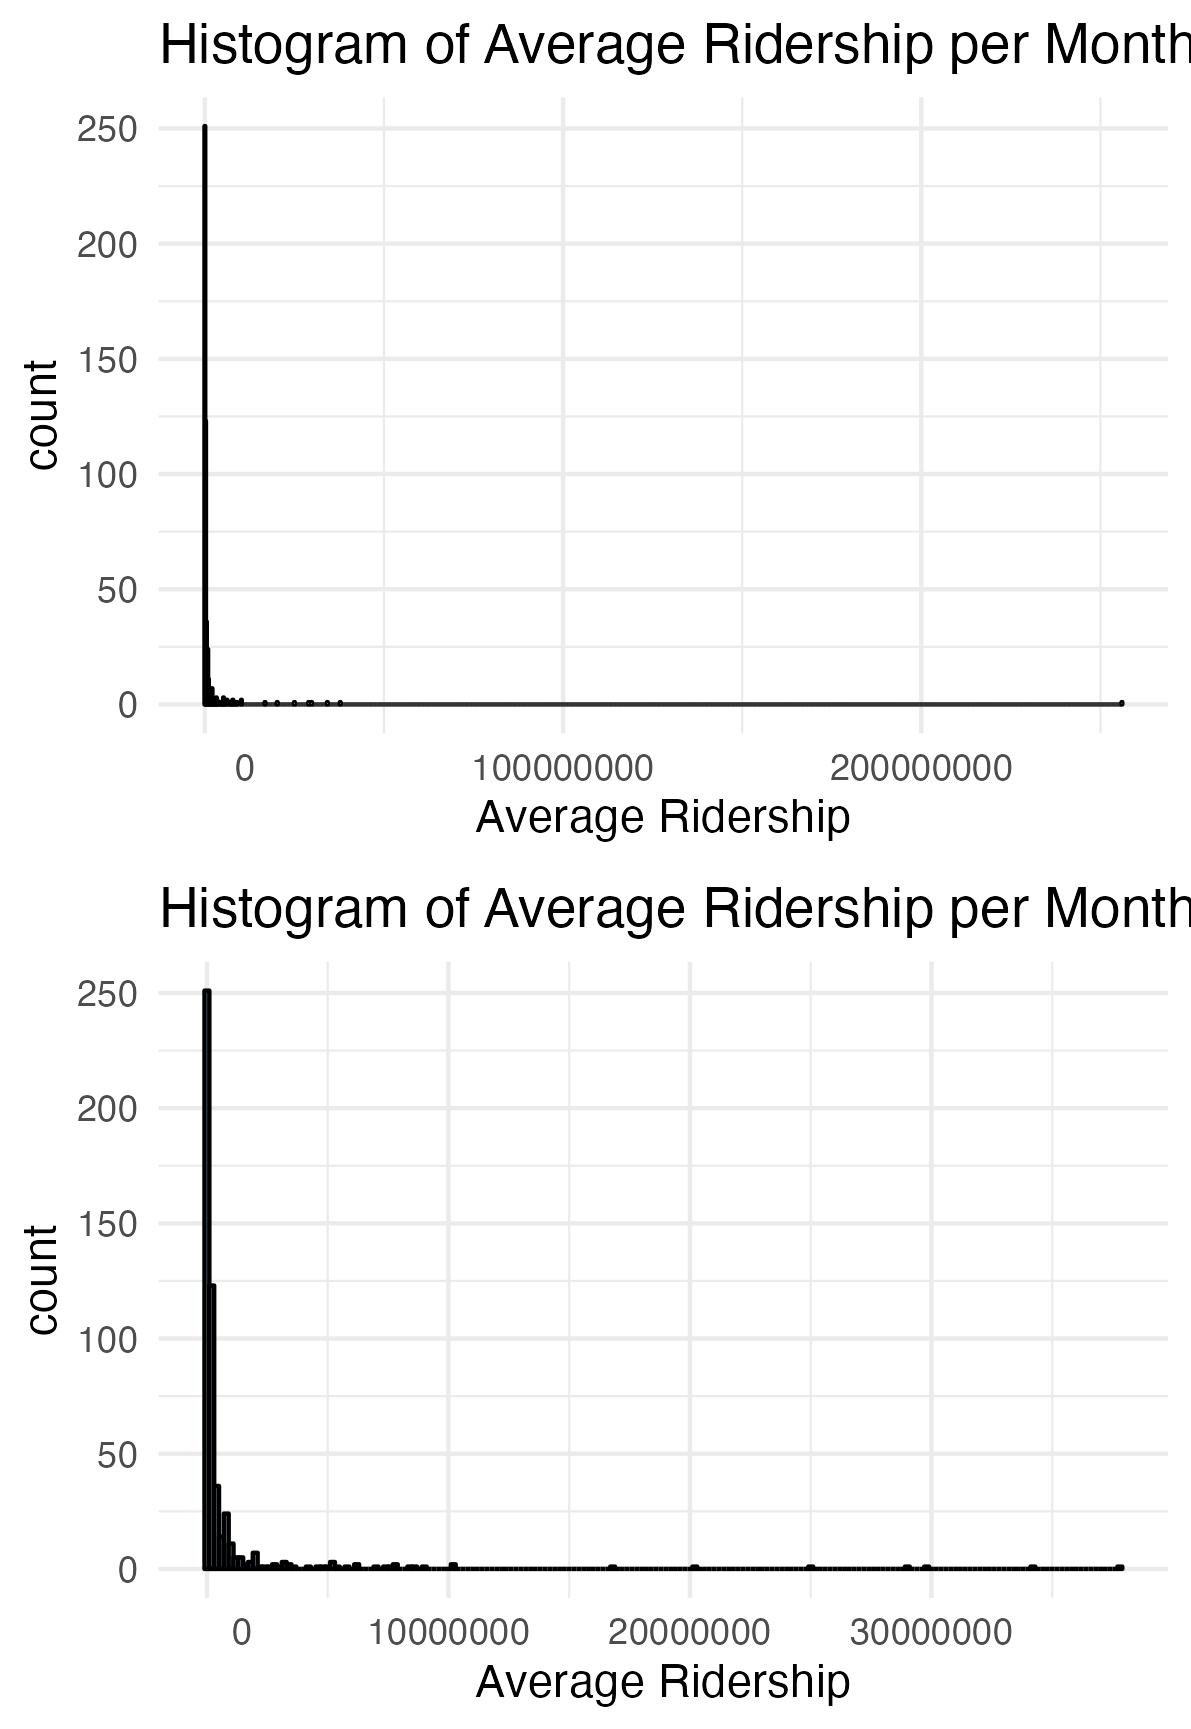
\includegraphics[width=0.8\textwidth]{avg_rides_per_agency.png} % Adjust width as needed
    \caption{Average rides per month (bin of 200,000). Bottom histogram does not include NYC}
\end{figure}
\begin{figure}[H]
    \centering
    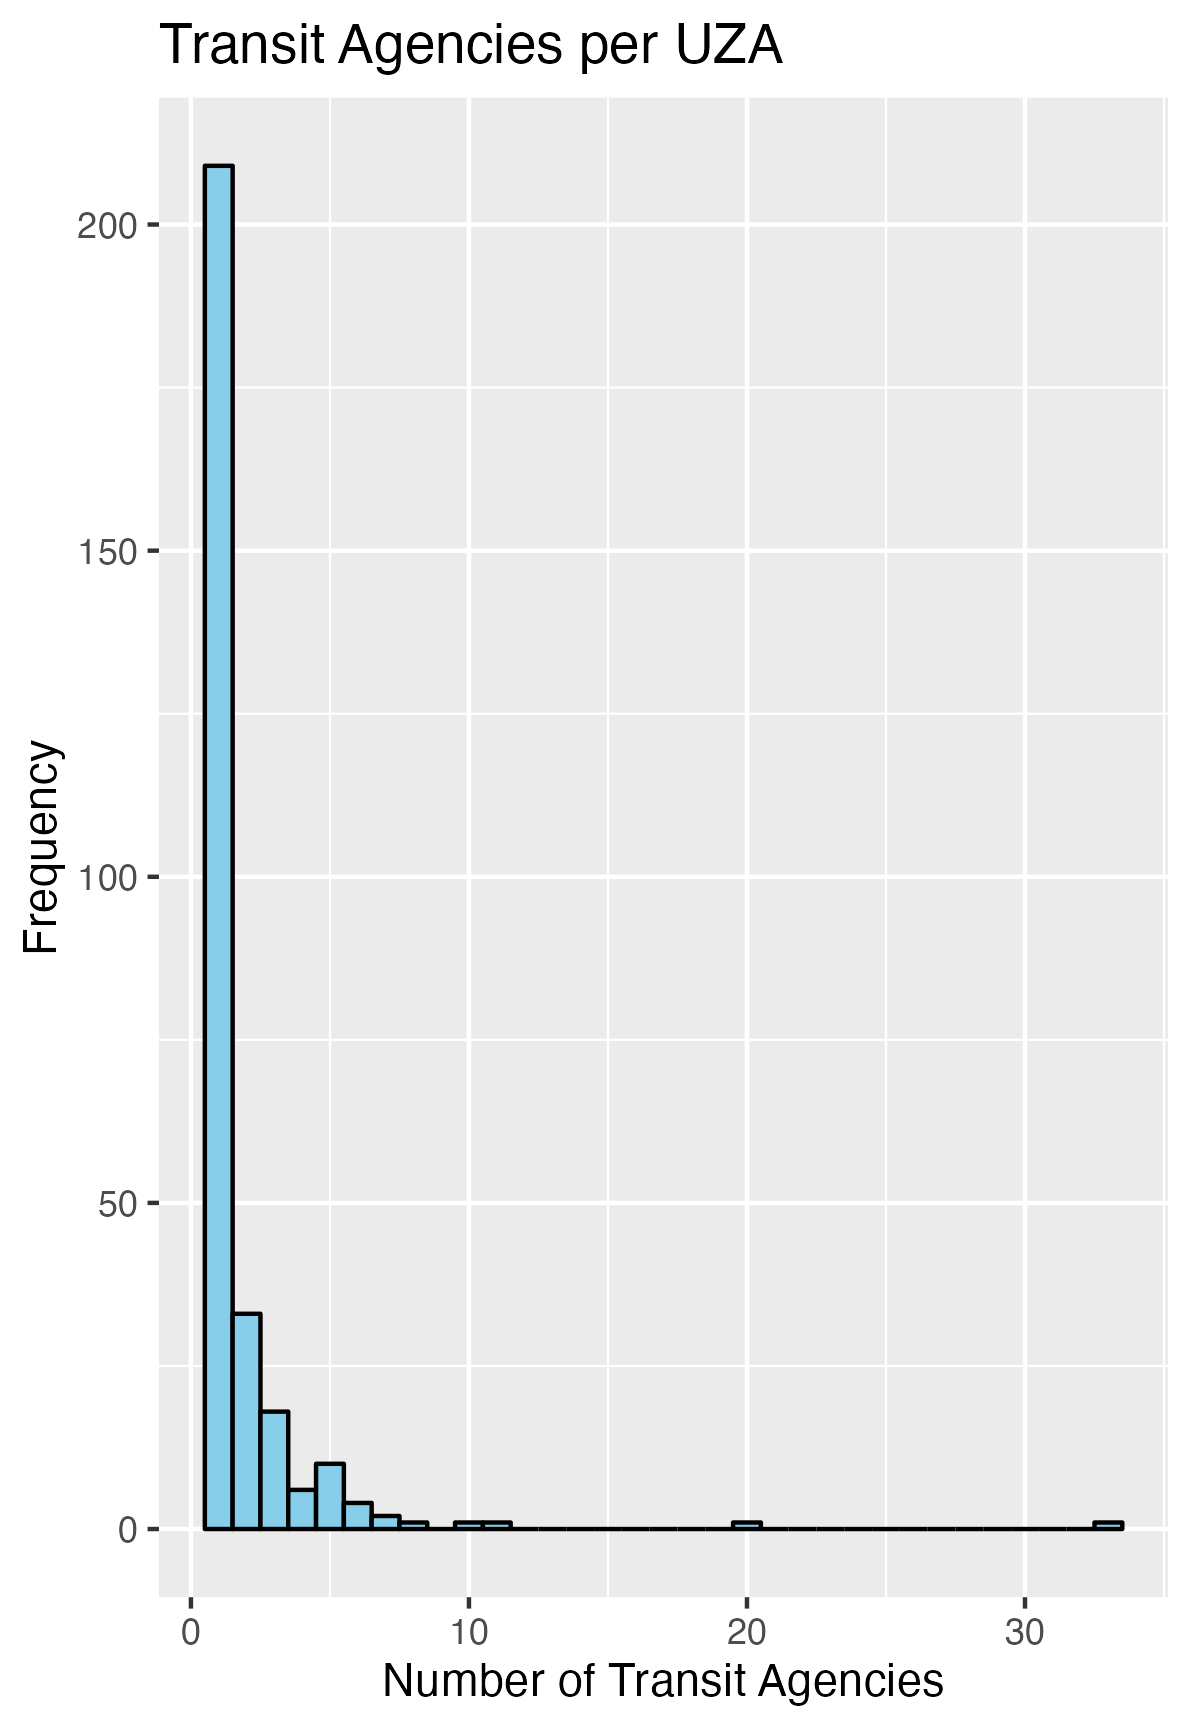
\includegraphics[width=0.8\textwidth]{avg_agencies_uza.png} % Adjust width as needed
    \caption{Average number of agencies per UZA}
\end{figure}
\begin{figure}[H]
    \centering
    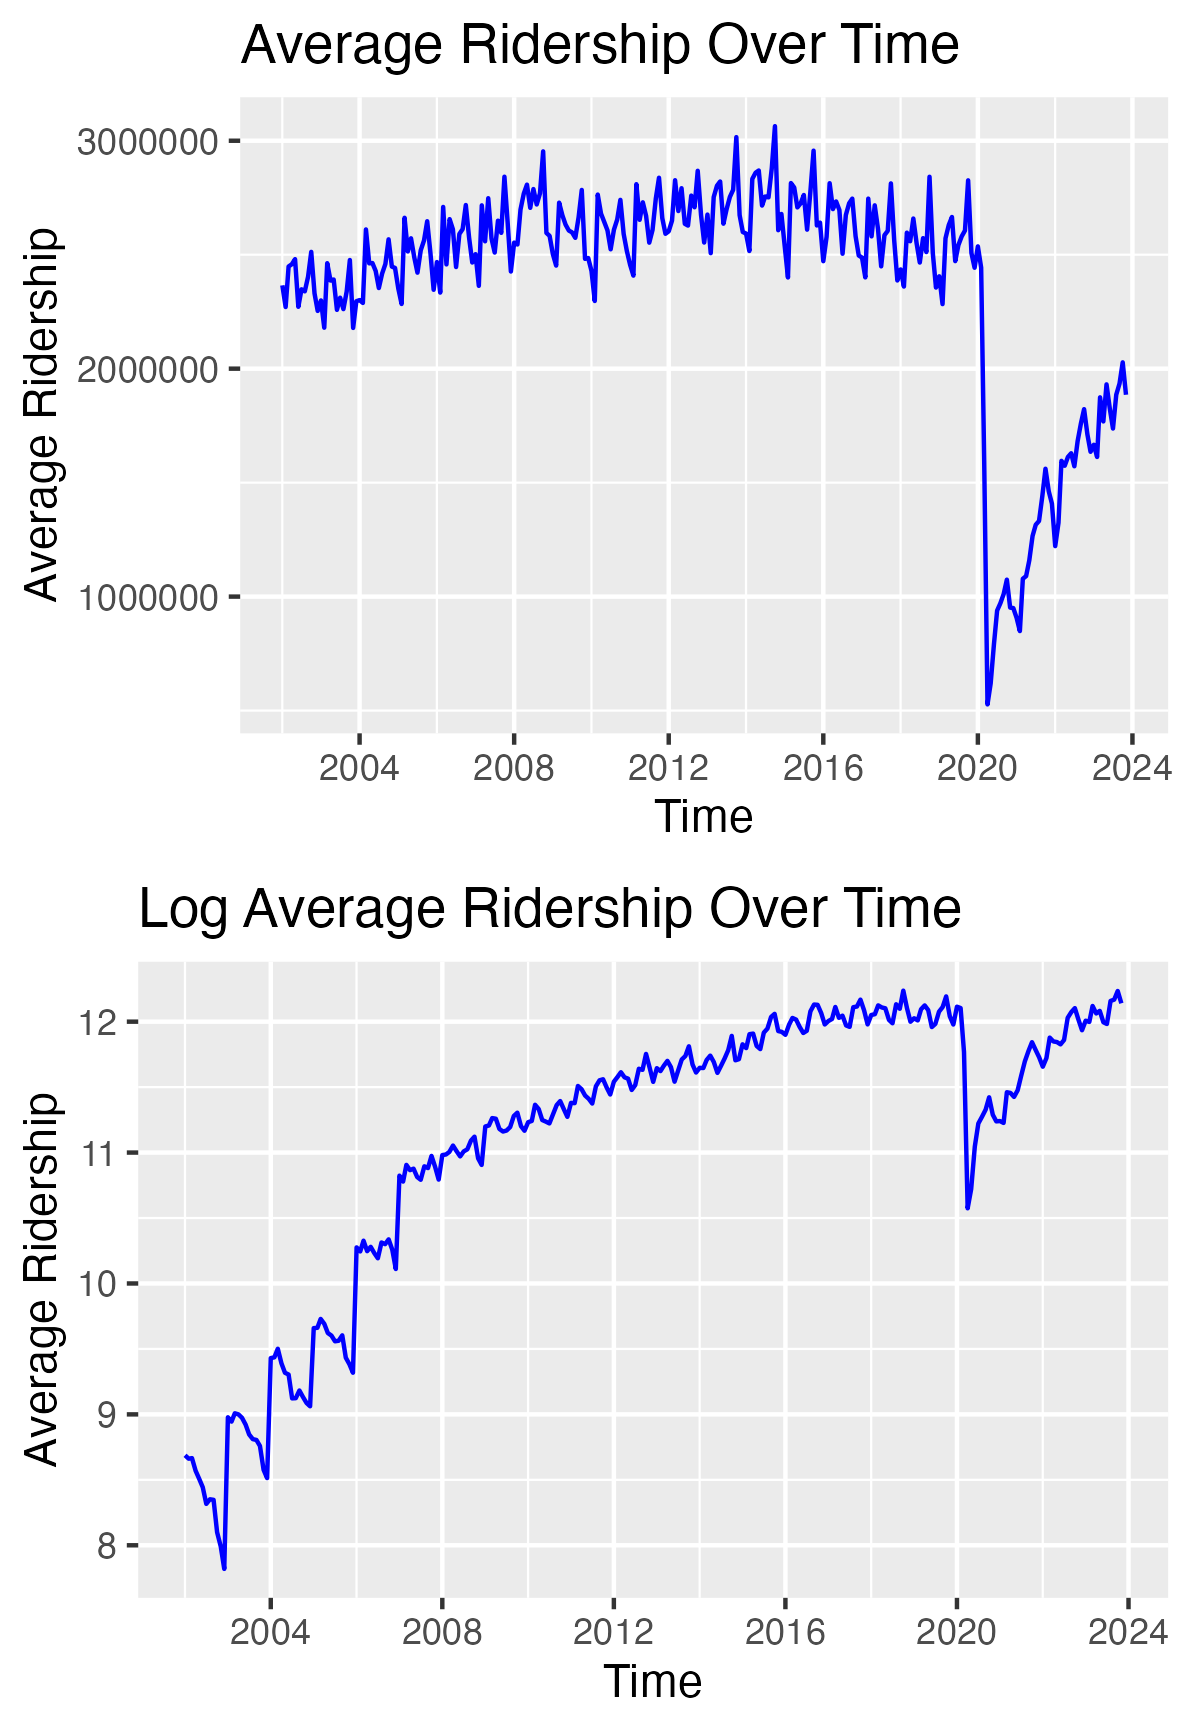
\includegraphics[width=0.8\textwidth]{avg_ridership_over_time.png} % Adjust width as needed
    \caption{Ridership over time}
\end{figure}
\begin{figure}[H]
    \centering
    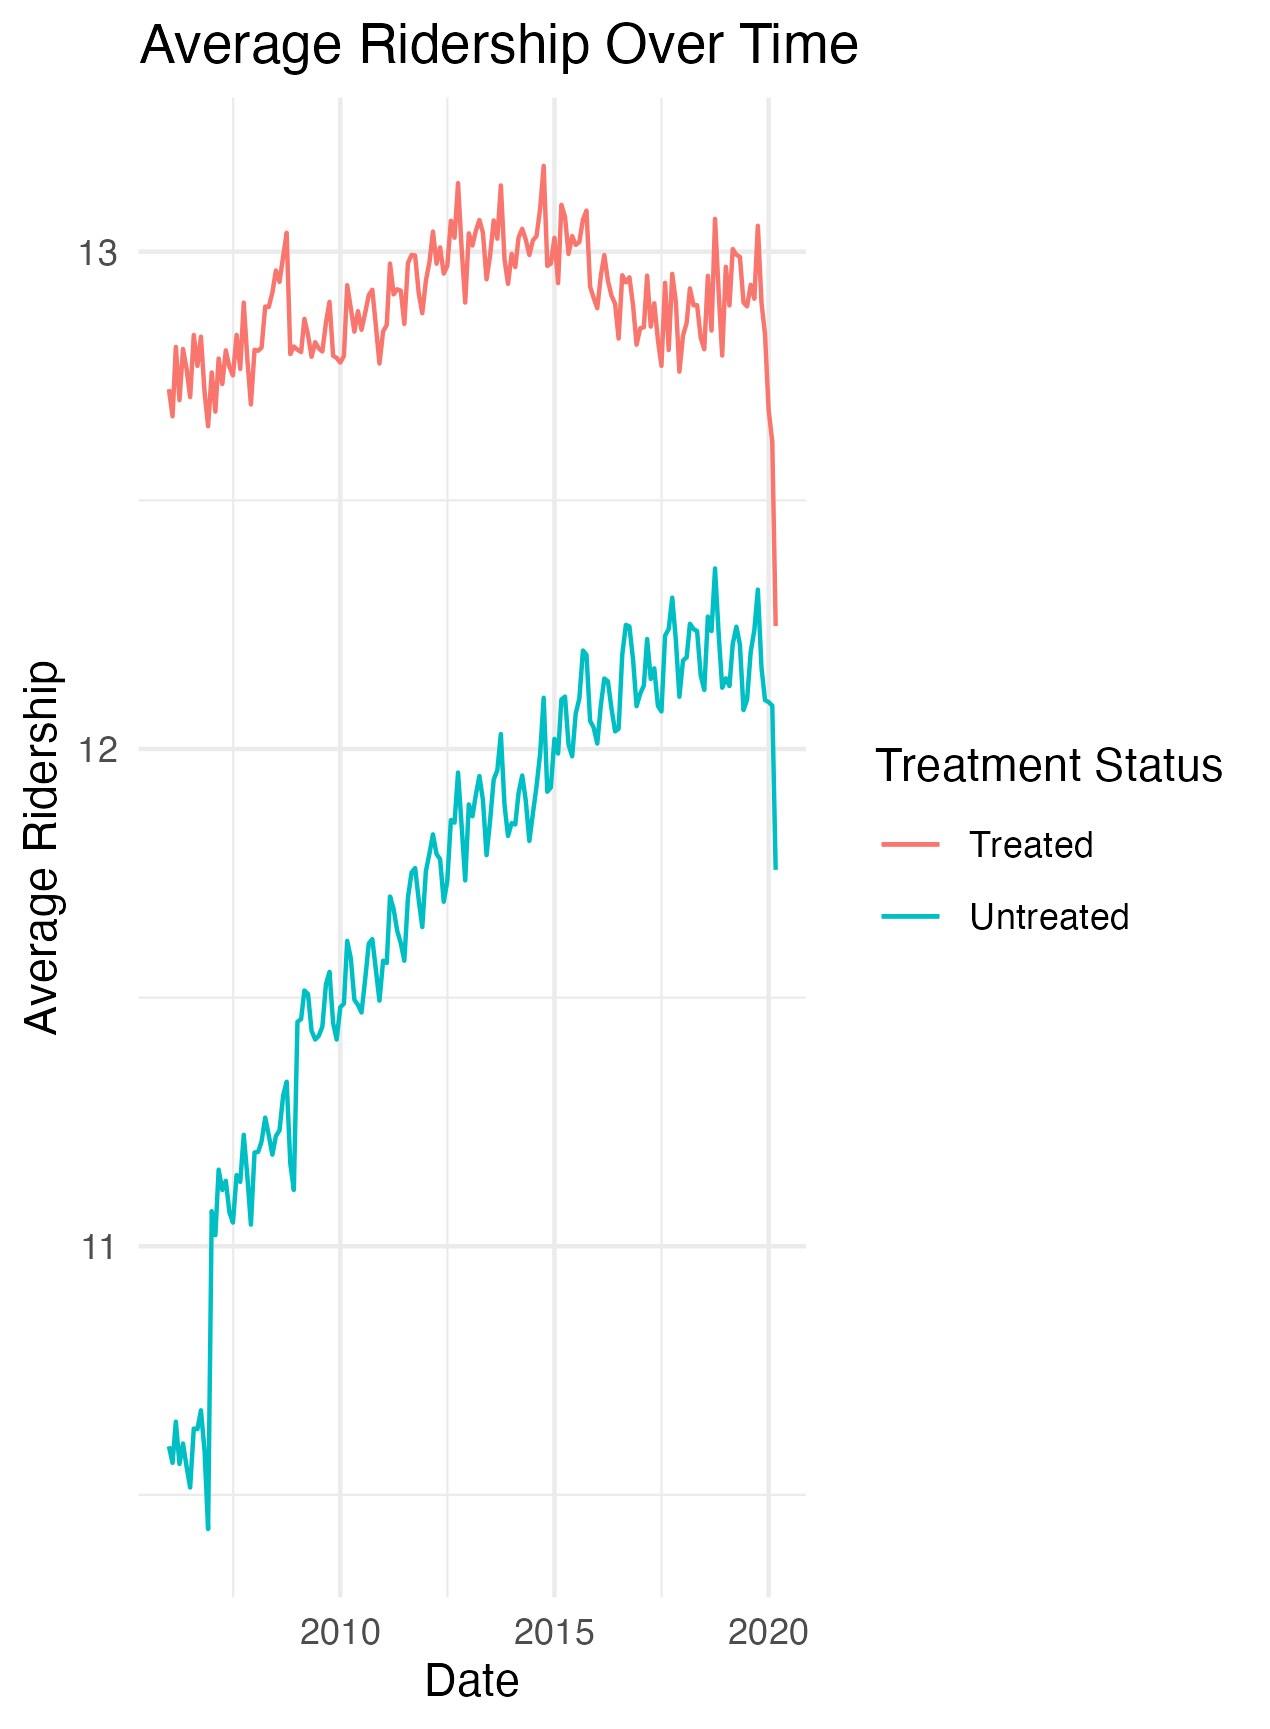
\includegraphics[width=0.8\textwidth]{avg_ridership_over_time_treated.png} % Adjust width as needed
    \caption{Ridership over time, Treated vs. Control}
\end{figure}
\begin{figure}[H]
    \centering
    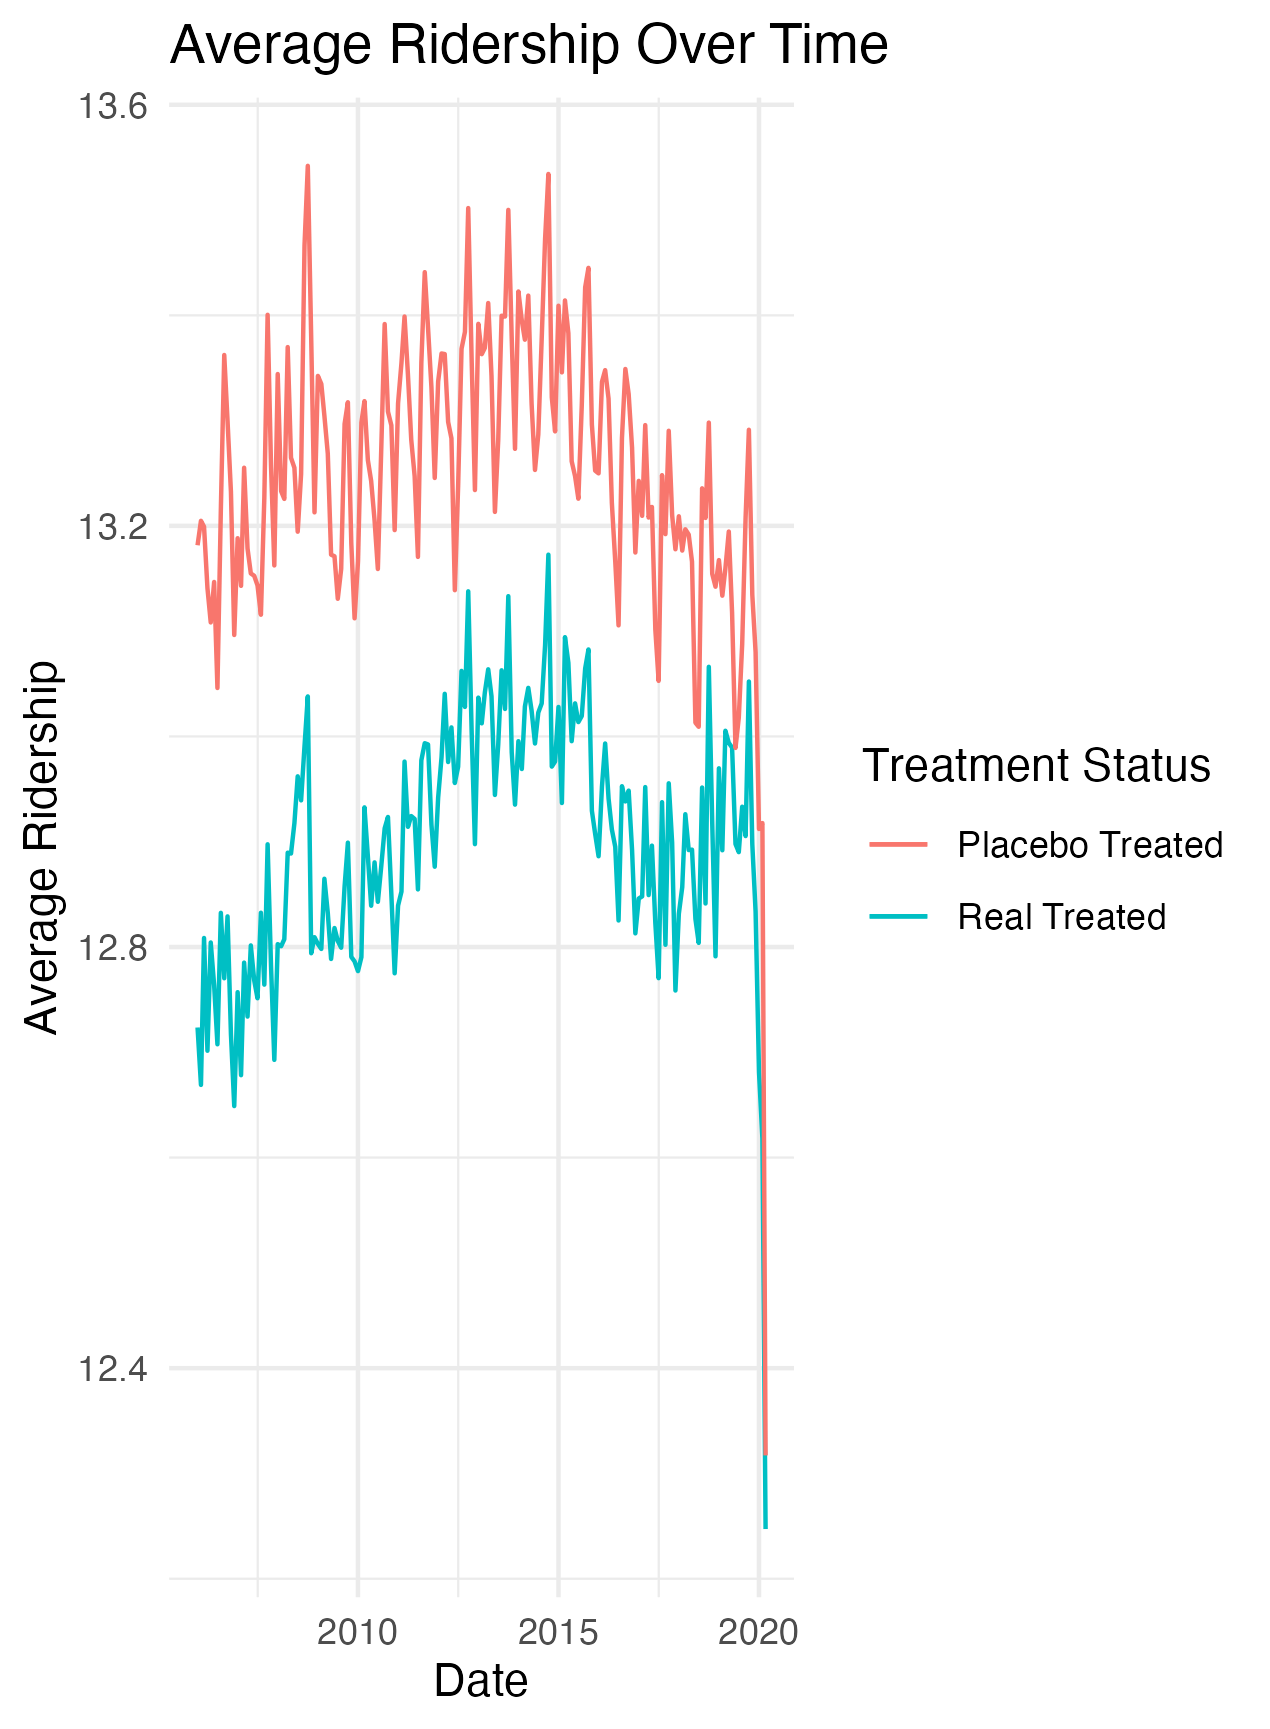
\includegraphics[width=0.8\textwidth]{avg_ridership_over_time_placebo.png} % Adjust width as needed
    \caption{Ridership over time, Treated vs. Placebo}
\end{figure}
\begin{figure}[H]
    \centering
    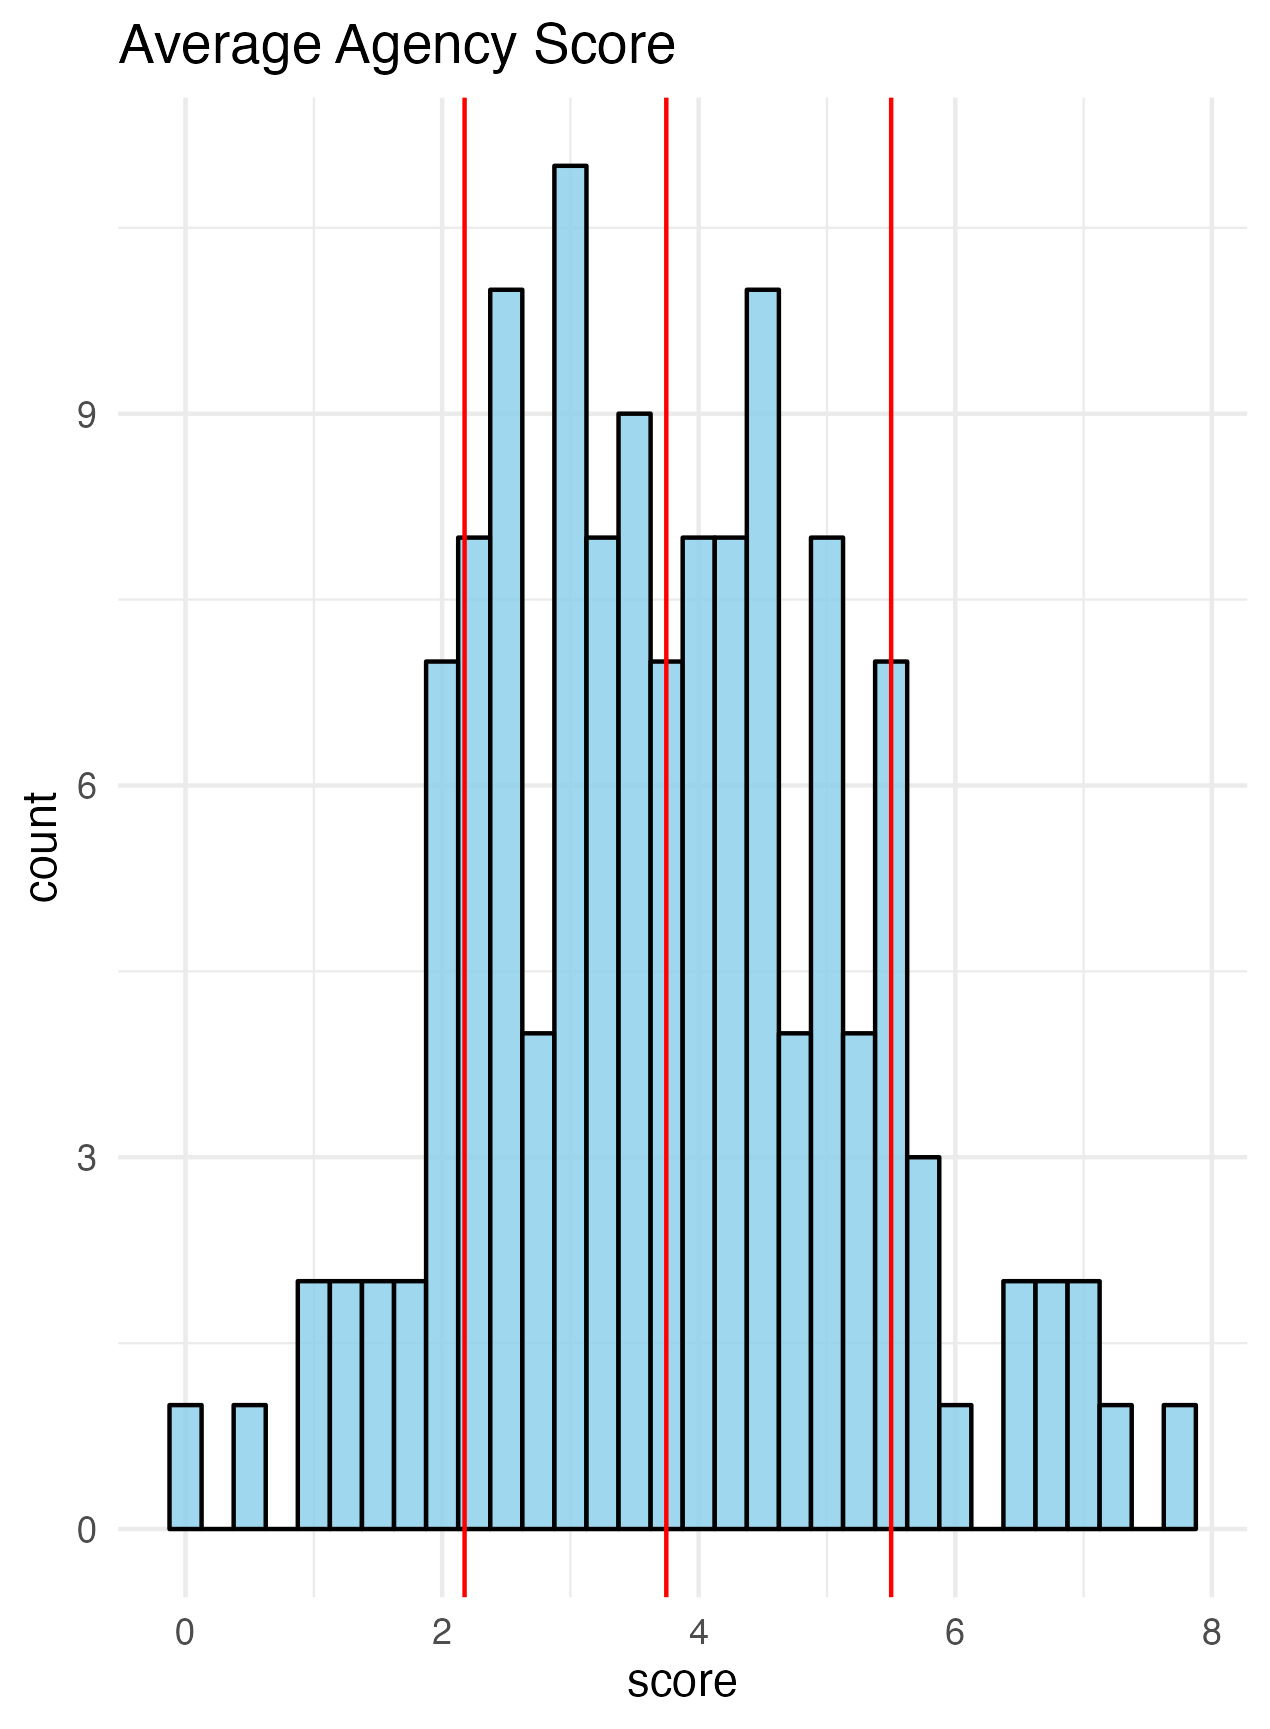
\includegraphics[width=0.8\textwidth]{avg_agency_score.png} % Adjust width as needed
    \caption{Distribution of agency scores}
\end{figure}
\textbf{Notes}
According to AllTransit (through email correspondence), a score of 7+ is a "good" transit system by US standards. This is done at UZA level, not agency level so should be used with total ridership, not agency ridership
\begin{figure}[H]
    \centering
    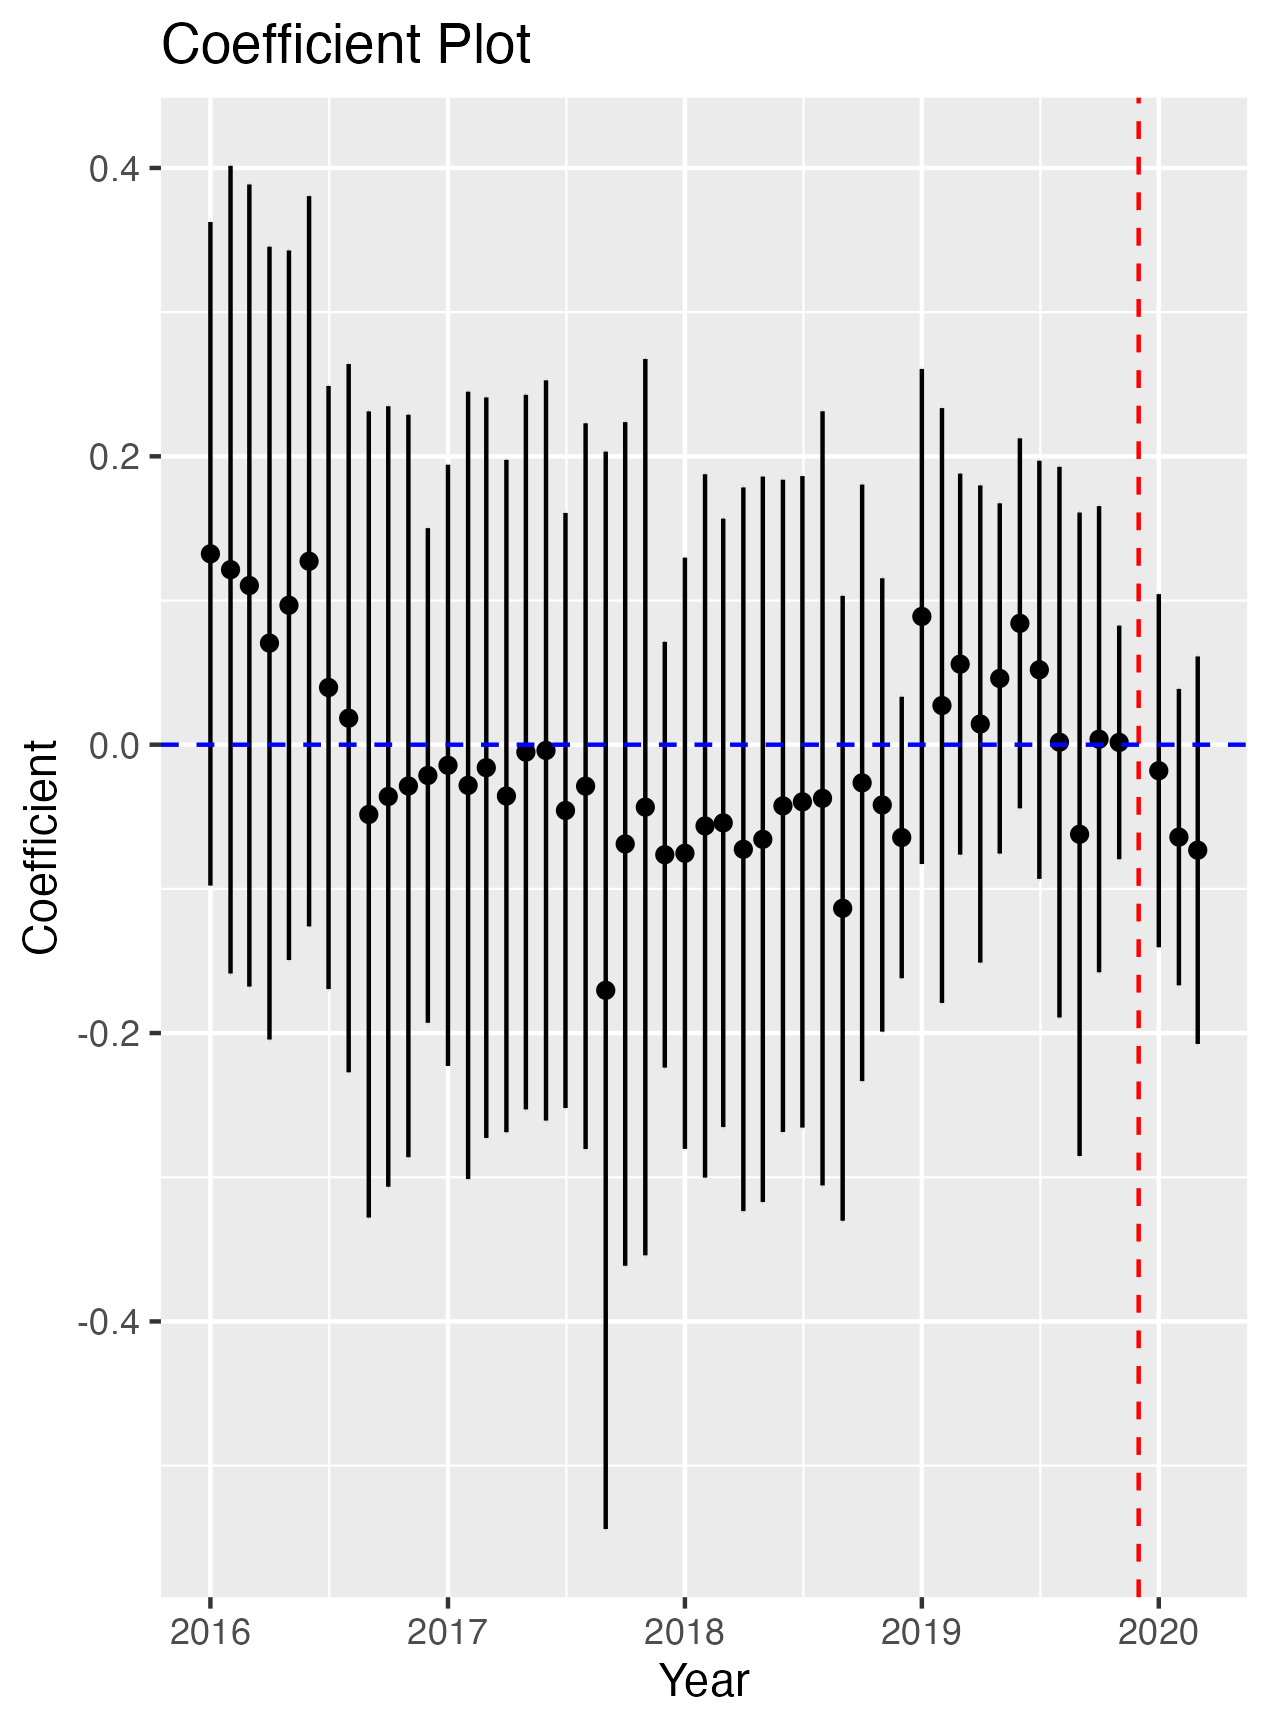
\includegraphics[width=0.8\textwidth]{coeff_plot.png} % Adjust width as needed
    \caption{Coefficient plot of log(ridership)}
\end{figure}
\textbf{Notes}
From 2016-01-01 to 2020-03-01



\end{document}